\documentclass[12pt]{article}

%%%%%%%%%%%%%%%%%%%%%%%%%%%%%%%%%%%%%%%%%%%%%%%%%%%%%%%%%%%%%%%%%%%%%%%%
%% Customizações do abnTeX2 (http://abnTeX2.googlecode.com)           %%
%% para a Universidade Estadual do Ceara - UECE                       %%
%%                                                                    %%
%% This work may be distributed and/or modified under the             %%
%% conditions of the LaTeX Project Public License, either version 1.3 %%
%% of this license or (at your option) any later version.             %%
%% The latest version of this license is in                           %%
%%   http://www.latex-project.org/lppl.txt                            %%
%% and version 1.3 or later is part of all distributions of LaTeX     %%
%% version 2005/12/01 or later.                                       %%
%%                                                                    %%
%% This work has the LPPL maintenance status `maintained'.            %%
%%                                                                    %%
%% The Current Maintainer of this work is Thiago Nascimento           %%
%%                                                                    %%
%% Project available on: https://github.com/thiagodnf/uecetex2        %%
%%                                                                    %%
%% Further information about abnTeX2                                  %%
%% are available on http://abntex2.googlecode.com/                    %%
%%                                                                    %%
%%%%%%%%%%%%%%%%%%%%%%%%%%%%%%%%%%%%%%%%%%%%%%%%%%%%%%%%%%%%%%%%%%%%%%%%

% \documentclass[
%     a4paper,          % Tamanho da folha A4
%     12pt,             % Tamanho da fonte 12pt
%     chapter=TITLE,    % Todos os capitulos devem ter caixa alta
%     section=TITLE,    % Todas as secoes devem ter caixa alta
%     oneside,          % Usada para impressao em apenas uma face do papel
%     english,          % Hifenizacoes em ingles
%     spanish,          % Hifenizacoes em espanhol
%     brazil            % Ultimo idioma eh o idioma padrao do documento
% ]{abntex2}



% Importações de pacotes
\usepackage[utf8]{inputenc}                         % Acentuação direta
\usepackage[T1]{fontenc}                            % Codificação da fonte em 8 bits
\usepackage{graphicx}                               % Inserir figuras
\usepackage{amsfonts, amssymb, amsmath}             % Fonte e símbolos matemáticos
\usepackage{booktabs}                               % Comandos para tabelas
\usepackage{verbatim}                               % Texto é interpretado como escrito no documento
\usepackage{multirow, array}                        % Múltiplas linhas e colunas em tabelas
\usepackage{indentfirst}                            % Endenta o primeiro parágrafo de cada seção.
\usepackage{listings}                               % Utilizar codigo fonte no documento
\usepackage{xcolor}
\usepackage{microtype}                              % Para melhorias de justificação?
\usepackage[portuguese,ruled,lined]{algorithm2e}    % Escrever algoritmos
\usepackage{algorithmic}                            % Criar Algoritmos
\usepackage{float}                                  % Utilizado para criação de floats
\usepackage{amsgen}
\usepackage{lipsum}                                 % Usar a simulação de texto Lorem Ipsum
%\usepackage{titlesec}                               % Permite alterar os títulos do documento
\usepackage{tocloft}                                % Permite alterar a formatação do Sumário
\usepackage{etoolbox}                               % Usado para alterar a fonte da Section no Sumário
\usepackage[nogroupskip,nonumberlist,acronym]{glossaries}                % Permite fazer o glossario
\usepackage{caption}                                % Altera o comportamento da tag caption
\usepackage[num, abnt-emphasize=bf, bibjustif, recuo=0cm, abnt-etal-cite=2, abnt-etal-list=0]{abntex2cite}  % Citações padrão ABNT
%\usepackage[bottom]{footmisc}                      % Mantém as notas de rodapé sempre na mesma posição
%\usepackage{times}                                 % Usa a fonte Times
\usepackage{mathptmx}                               % Usa a fonte Times New Roman
%\usepackage{lmodern}                               % Usa a fonte Latin Modern
%\usepackage{subfig}                                % Posicionamento de figuras
%\usepackage{scalefnt}                              % Permite redimensionar tamanho da fonte
%\usepackage{color, colortbl}                        % Comandos de cores
%\usepackage{lscape}                                % Permite páginas em modo "paisagem"
%\usepackage{ae, aecompl}                           % Fontes de alta qualidade
%\usepackage{picinpar}                              % Dispor imagens em parágrafos
%\usepackage{latexsym}                              % Símbolos matemáticos
%\usepackage{upgreek}                               % Fonte letras gregas
\usepackage{appendix}                               % Gerar o apendice no final do documento
\usepackage{paracol}                                % Criar paragrafos sem identacao
\usepackage{lib/uecetex2}		                    % Biblioteca com as normas da UECE para trabalhos academicos
\usepackage{pdfpages}                               % Incluir pdf no documento
\usepackage{amsmath}                                % Usar equacoes matematicas

\usepackage{hyperref}

\usepackage{glossaries}

\usepackage{enumerate}
\usepackage{enumitem}

\renewcommand{\ABNTEXchapterfontsize}{\normalsize}

\renewcommand{\ABNTEXsectionfontsize}{\normalsize}

% Organiza e gera a lista de abreviaturas, simbolos e glossario
\makenoidxglossaries

% Gera o Indice do documento
\makeindex

     
\sloppy

\title{Processamento das Sequências Obtidas com Equipamentos de \gls{ngs}}

\author{Diego Frias e Mauricio Souza Menezes\\}
\address{Departamento de Ciências Exatas e da Terra, Campus I\\
Universidade do Estado da Bahia (UNEB)\\
Salvador, Bahia, Brasil.
  \email{mauriciosm95@gmail.com}
}

\begin{document}

\newacronym{ufm}{UFM}{Universal Feature Method}
\newacronym{ngs}{NGS}{Sequenciamento de Nova Geração}
\newacronym{ed}{ED}{Estruturas de Dados}
\newacronym{rs}{RS}{Revisão Sistemática}
\newacronym{cafe}{CAFe}{Comunidade Acadêmica Federada}
\newacronym{ieee}{IEEE}{Institute of Electrical and Electronic Engineers}
\newacronym{scielo}{SciELO}{Scientific Electronic Library Online}

\maketitle

\begin{resumo}
    Este documento tem como objetivo descrever o contexto da pesquisa, com vistas a definir melhor o escopo do projeto. Possíveis questões de pesquisa são elaboradas ao longo do texto, para uma posterior seleção e generalização.
\end{resumo}


\begin{abstract}
    \begin{otherlanguage}{english}
        This document aims to describe the context of the research, in order to better define the scope of the project. Possible research questions are elaborated throughout the text, for later selection and generalization.
    \end{otherlanguage} 
\end{abstract}


\section{Introdução}

Começamos listando algumas especificidades do \gls{ngs}:
\begin{itemize}
    \item Pode ser aplicado para sequenciar DNA (dupla hélice) ou RNA (hélice única) mas, não os dois ao mesmo tempo.
    \item O DNA/RNA na amostra é fragmentado de forma aleatória, acoplando-se adaptadores a um ou os dois extremos de cada fragmento. Estes adaptadores fixam o fragmento à cela de sequenciamento e são parcial ou totalmente sequenciados, o que exige uma etapa inicial de processamento para retirar os adaptadores.
    \item A amostra pode conter diversos tipos de material genético, além do DNA/RNA que deseja ser sequenciado, como é o caso de amostras de sangue para sequenciamento de vírus, nas quais pode haver outros vírus e DNA/RNA das distintas células do sangue. De acordo com isto é necessário filtrar todas as sequências que não são do vírus em estudo.
    \item Nas amostras meta-genômicas existem fragmentos de DNA/RNA de genomas/transcriptomas de múltiplos organismos, o que requer um processamento diferenciado. Neste trabalho não abordaremos sequenciamento metagenômico.
    \item Podemos diferenciar dois tipos de problemas de sequenciamento: 
    \begin{enumerate}
        \item Sequenciamento de novas espécies, em cujo caso é preciso construir o genoma dela a partir da sobreposição dos fragmentos. Este problema é conhecido como {\it{de novo assembly}}. Neste problema, uma vez montado o genoma, é necessário fazer a anotação do mesmo. A anotação consiste em identificar o início e fim de cada gene. No caso dos eucariotos, como os genes podem conter introns, é necessário identificar o início e o fim de cada intron, para poder concatenar os exons (regiões codificantes) e obter as sequências de aminoácido das proteínas codificada pelos genes. No caso de procariotos o problema é mais simples pois os genes não possuem (em geral) introns. No caso dos vírus, que possuem genoma muito compacto, muitos dos genes são encadeados em quadros abertos de leitura (Open Reading Frame - ORF) que codificam vários genes. As ORFs são transcritas e traduzidas de uma única vez, ocorrendo a separação das proteínas após a tradução num processo conhecido como clivagem da cadeia polipeptídica. Este processo de clivagem é controlado por proteínas não estruturais (NSP) codificadas por outras ORFs que são traduzidas primeiro para poder produzir as proteínas estruturais virais. O resultado deste tipo de projeto de sequenciamento é um genoma anotado. Este genoma anotado pode ser usado como referência no próximo tipo de projeto de sequenciamento, descrito a seguir.
        
        \item Sequenciamento de espécies conhecidas dispondo de um genoma de referência anotado. Este é o caso nos projetos de sequenciamento genômico de vírus para estudar a evolução dos mesmos e o surgimento de novas espécies (vigilância biomolecular de patógenos). O resultado imediato destes projetos de sequenciamento é uma listagem de mutações (mudanças pontuais de aminoácidos) entre o genoma sequenciado e o de referência. Os arquivos com a listagem das mutações tem extensão .vcf do termo em inglês {\it{Variant Calling File}}. Paralelamente, estes projetos adicionam novos genomas anotados à base de dados, o que permite fazer uma análise filogenética das cepas sequenciadas em diferentes momentos e localidades, o que é uma poderosa ferramenta de análise da evolução viral. 
        Na figura \ref{fig:pipeline_1} mostramos o pipeline genérico e nas figuras \ref{fig:pipeline_2} e \ref{fig:pipeline_3} dois pipelines mais detalhados.
        \begin{figure}[h!]
            \centering
            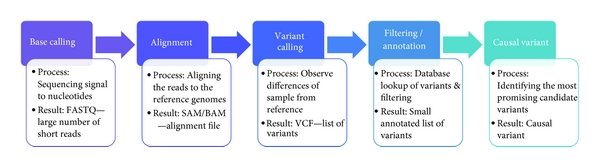
\includegraphics[scale=2.3]{./figuras/Next-generation-sequencing-bioinformatics-workflow_W640}
            \caption{Pipeline simplificado}
            \label{fig:pipeline_1}
        \end{figure}
        
        \begin{figure}[h!]
            \centering
            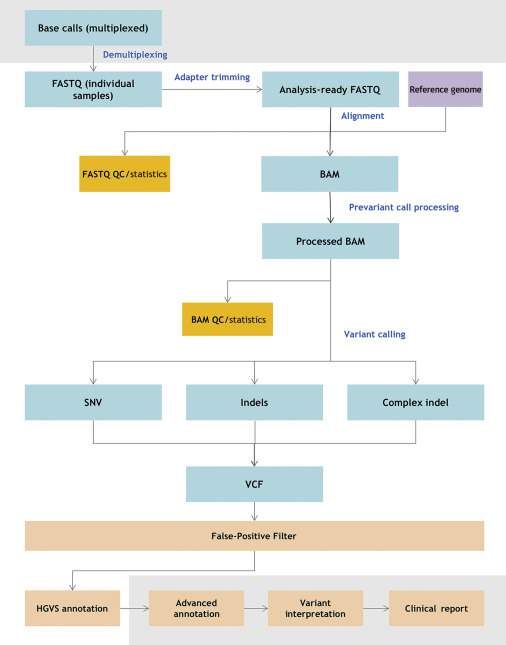
\includegraphics[scale=1.0]{./figuras/ngs_pipeline}
            \caption{Typical variant calling bioinformatics pipeline}
            \label{fig:pipeline_2}
        \end{figure}
        
         \begin{figure}[h!]
            \centering
            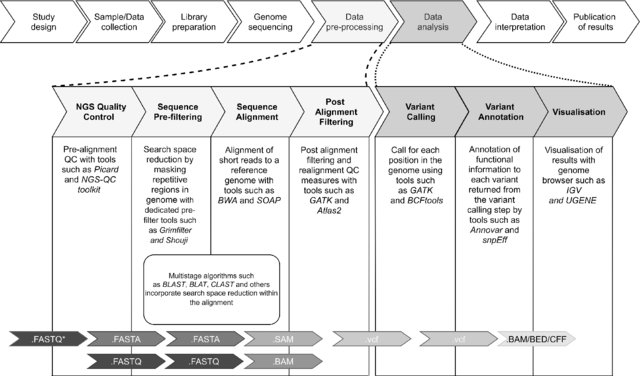
\includegraphics[scale=1.6]{./figuras/Typical-variant-calling-bioinformatics-pipeline-composed-of-steps-following-NGS_W640}
            \caption{Typical variant calling bioinformatics pipeline composed of steps following NGS sequencing leading to the visualization of data is presented in the middle panel. The variant calling bioinformatics pipeline is contained within the data pre-processing and data analysis stages of a much larger bioinformatics-based research study as illustrated in the upper panel. Data file formats at each step are presented in the lower panel (Al Kawam et al., 2017; Lightbody et al., 2019). *Platform-specific raw sequence output either .BAM or .FASTQ or .HDF5 (NCBI, 2019).}
            \label{fig:pipeline_3}
        \end{figure}
        
        \item O de {\it{novo assembly}} é um problema NP-hard, mas tem sido desenvolvidos métodos baseados em grafos (Eulerianos \url{https://en.wikipedia.org/wiki/Eulerian_path}, Hamiltonianos \url{https://en.wikipedia.org/wiki/Hamiltonian_path} e de Bruijn ( \url{https://en.wikipedia.org/wiki/De_Bruijn_graph} e \url{https://web.archive.org/web/20141030124239/http://www.homolog.us/Tutorials/index.php?p=2.1&s=1})), bastante eficientes. 
        
        Na figura \ref{fig:assembly} mostramos o pipeline genérico de um de novo assembly.
        
        \begin{figure}[h!]
            \centering
            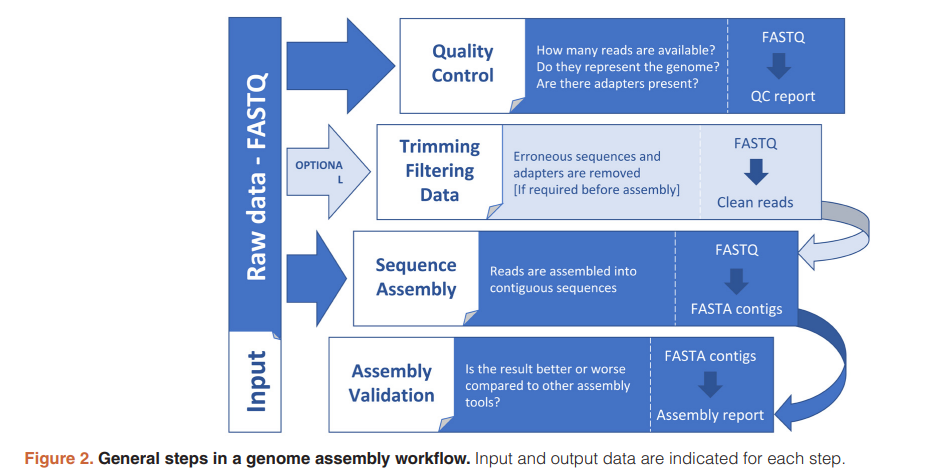
\includegraphics[scale=0.65]{./figuras/pipeline_assembly}
            \caption{Pipeline genérico do {\it{de novo assembly}}}
            \label{fig:assembly}
        \end{figure}
        
        Depois da montagem do genoma (contigs) se procede à anotação dos mesmos: identificação das sequências de DNA/RNA que codificam as proteínas e os RNAs funcionais. Na figura \ref{fig:annotation} mostramos o pipeline genérico desta fase. Observe o uso de métodos ab-initio, como o \gls{ufm}.  
        
        \begin{figure}[h!]
            \centering
            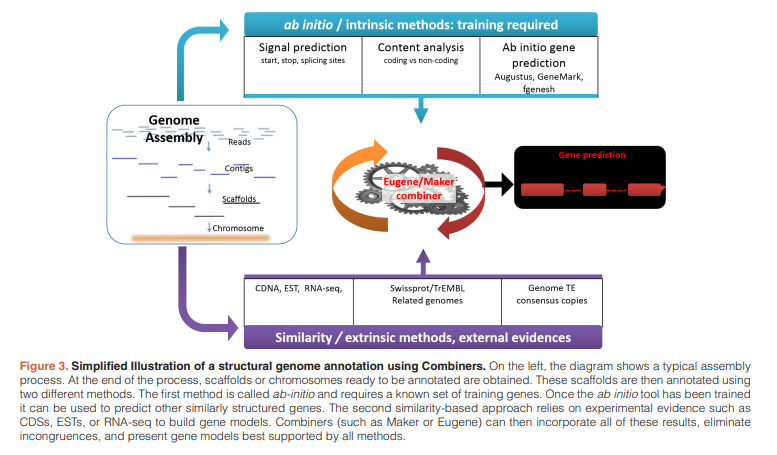
\includegraphics[scale=0.85]{./figuras/pipeline_annotation}
            \caption{Pipeline genérico da anotação  de genomas}
            \label{fig:annotation}
        \end{figure}
        
        
        \underline{Comentários:} 
        
        (1) Pelo que tenho visto, todas as ferramentas para {\it{de novo assembly}} trabalham com sequências de nucleotídeos, ou seja, alinham sequências codificantes e não codificantes. Então precisa ver se alguma ferramenta trabalha com sequências de aminoácidos (alinhando apenas sequências codificantes), porque \gls{ufm} traduz os fragmentos de nucleotídeos para fragmentos de aminoácidos. Neste cenário, que percentual dos fragmentos sequenciados com diferentes técnicas \gls{ngs} são considerados codificantes pelo \gls{ufm} para diferentes virus, pode ser uma questão de pesquisa. 
        
        (2) Uma peculiaridade de trabalharmos com \gls{ufm} é que o {\it{de novo assembly}} pode ser "focado" apenas nos genes, descartando-se automaticamente as regiões não codificantes do genoma sendo sequenciado. Quanto mais barato e efetivo seria? Acho que não vai ser uma das suas questões de pesquisa. Será de um trabalho futuro. 
        
        \item O alinhamento de fragmentos de comprimento médio $f$, contra um genoma de referência de comprimento $g$ é o método para processar sequências de espécies conhecidas. Neste contexto, uma das suas perguntas de pesquisa será: quais métodos são os mais utilizados e qual o custo computacional dos mesmos em função de $f$ e $g$.
        
        \underline{Comentários:}
        
        (1) Quando um fragmento é alinhado ao genoma de referência, é necessário consultar a anotação para determinar se o fragmento é pelo menos parcialmente codificante, e em caso positivo identificar a sequência de aminoácidos codificada pelo fragmento. Uma das suas perguntas de pesquisa pode ser: Qual é a complexidade computacional desse processo, em função de $f$. 
        
        (2) O \gls{ufm} não é capaz de identificar partes codificantes nos fragmentos. Esperamos que se uma boa parte do fragmento for codificante, então ele irá indicar esse fragmento como codificante e gerará uma sequência de aminoácidos para todo o fragmento. Como no caso excepcional analisado, apenas uma parte do fragmento é codificante, a cadeia de aminoácidos geradas pelo \gls{ufm} estará apenas parcialmente correta. Como podemos lidar com isto no caso dos sequenciamentos com referência e {\it{de novo assembly}}?. 
        
        Outra pergunta a ser respondida é qual é o limiar (número de nucleotídeos codificantes) para que \gls{ufm} identifique um fragmento como codificante? De fato, o problema é mais complexo. Podemos identificar que com 200 nucleotídeos para cima ele tem uma taxa X (favorável) de acerto, mas se colocamos em um dos extremos "n" \  bases não codificantes, como se comporta o método? Ou seja, garantido que a parte codificante tem o número mínimo de nucleotídeos, como varia a taxa de acerto quando se acrescenta um percentual de sequência não codificante em um dos extremos? Depende do extremo, direito ou esquerdo?
        
        \item Uma alternativa para identificar as mutações no arquivo de sequenciamento limpo de artefatos (obter o VCF), é alinhar cada fragmento ao genoma de referência usando blast. Uma versão do blast foi desenvolvida especificamente para esta tarefa (diamond  blast). Neste contexto surgem 3 questões de pesquisa a serem respondidas:
        
        (1) Quão exato é \gls{ufm} na detecção de sequências codificantes
        
        (2) Em caso positivo acima, quão mais rápido é \gls{ufm} que diamond blast.
        
        (3) Se usando diamond blast como pós-processamento da saída de \gls{ufm} (para excluir falsos positivos)  se consegue um processamento otimizado em velocidade e qualidade?.
        
    \end{enumerate}
    
\end{itemize}

\section{Integração do \gls{ufm} nos pipelines}

Primeiro devemos notar que \gls{ufm} é um método ab-initio para identificação de CDSs. Mas especificamente, para:
\begin{enumerate}
    \item Classificar sequências de nucleotídeos de entrada em codificante ou não codificante, e
    \item No caso codificante, identifica o quadro de leitura permitindo gerar como saída a sequência de aminoácidos (potencialmente) codificada pela sequência de entrada.
\end{enumerate}
Neste ponto surgem algumas questões a serem respondidas:
\begin{enumerate}
    \item Existem diversos outros métodos ab-initio. Porque usar \gls{ufm}?
    
    A resposta precisa levar em conta: 
    \begin{enumerate}
        \item A acurácia
        \item O custo computacional, e 
        \item O custo de treinamento do modelo
    \end{enumerate}
    
    O cenário mais favorável é aquele no qual \gls{ufm} tem nenhum ou menor custo de treinamento do modelo, menor custo computacional e acurácia similar ou superior à do melhor método existente.
    
    \item Temos várias condicionantes do estudo comparativo a serem tratadas:
    
    \begin{enumerate}
        \item  Quantos outros métodos (códigos) ab-initio estão disponíveis para teste? 
    
        \item Vamos comparar com métodos que usam mais features (promoter, TSS, etc)? 
    
        \item Como vamos comparar \gls{ufm} com métodos que são capazes de detectar fragmentos codificantes na sequência de entrada?
    
        \item Quais datasets serão selecionados para a comparação: quantos e de quais espécies? Só de vírus? de quais vírus? quantos genomas de cada vírus?
    \end{enumerate}
  
\end{enumerate}
Em segundo lugar, a ideia original do trabalho não é usar \gls{ufm} como substituto de outros métodos ab-initio nos pipelines com passo de anotação de genes, o que não é descartado, senão introduzir \gls{ufm} como um passo de pré-processamento de sequências no início dos pipelines, transformando os passos seguintes do pipeline para tratar sequências de aminoácidos em vez de sequências de nucleotídeos. 

Neste ponto precisamos responder algumas questões:

\begin{enumerate}
    \item O que se espera com esta mudança?   
    
    Esperamos várias coisas que simplificam o processamento, sem perda excessiva de qualidade:
    
    \begin{enumerate}
        \item Redução significativa do número de reads a serem processados no pipeline, devido à filtragem de reads não codificantes? 
        
        \underline{Quanto é significativo?} > 30\%, 50\%, 70\%? 
        
        Vai depender da espécie. Por exemplo, no caso de vírus, devido à alta compactação do genoma, a maioria dos reads serão codificantes. Não serão codificantes reads nas pequenas regiões entre ORFs e no início e final do genoma. Já em eucariotos onde existem grandes regiões inter-gênicas e introns, a porção de reads não codificantes deve ser maioritária.
        
        \underline{Surge a pergunta:} Precisamos fazer um estudo comparativo do percentual de sequências filtradas por \gls{ufm} em diferentes tipos de genomas (espécies)? Quantas espécies? 
        
        \item Menor custo computacional 
        
        \begin{enumerate}
            \item (\underline{No caso de {\it{de novo assembly}}}) para fazer montagem de sequências de aminoácidos, 1/3 menores, do que de nucleotídeos?
            
             \underline{Surgem as perguntas}:
            \begin{enumerate}
                \item Quanto menor? Dá para estimar de forma analítica?
                \item Os códigos de assembly atuais permitem montar sequências de aminoácidos? 
                \item Em caso positivo, qual é o mais rápido (mais usado deles)? Como vamos testar o ganho de performance? Quais genomas, quantos?
                \item Em caso negativo, vamos construir um ensamblador com as duas variantes para o estudo? Vamos comparar o ensamblador de teste com outros de pratilheira para poder estender o resultado? BURACO NEGRO
            \end{enumerate} 
            
            \item (\underline{No caso de alinhamento contra referência}) para fazer alinhamento contra a referência de sequências de aminoácidos, 1/3 menores, do que de nucleotídeos?
         
        \underline{Surgem as perguntas}:
        \begin{enumerate}
            \item Quanto menor? Dá para estimar de forma analítica?
            \item Qual código de alinhamento de 2 sequências vamos usar para avaliar o ganho? Por qué?
            \item Como vamos testar o ganho de performance? Quais genomas, quantos?
        \end{enumerate} 
    \end{enumerate}
    \item Filtragem automática de mutações sinônimas, reduzindo o custo de construção do VCF.
     
     \underline{A redução é significativa?} > 30\%, 50\%, 70\%? 
        
    \underline{De quais fatores depende a redução?}
\end{enumerate}

\item Quais as desvantagens ou pontos fracos dessa abordagem que precisam ser estudados?

Numa análise preliminar vejo alguns pontos que precisamos acompanhar e avaliar no projeto:
\begin{enumerate}
    \item A acurácia de \gls{ufm} diminui com a redução do tamanho das sequências. 
    
    Então precisamos mapear os comprimentos médios e desvio padrão dos reads das distintas técnicas NGS para avaliar a acurácia com cada técnica. 
    
    \item \gls{ufm} foi desenhado para ter parâmetros fixos para todas as espécies, mas, estudos preliminares quer fiz com 2 vírus, mostraram necessidade de ajustar os parâmetros do modelo.  
    
    Eu explorei um método simples de ajuste de parâmetros que precisaria ser avaliado antes de inclui-lo como parte do pipeline.
    
    \underline{Perguntas:}
    
    \begin{enumerate}
        \item O ajuste paramétrico precisa ser realizado apenas para vírus, ou para outras espécies também. No caso de vírus, precisa ser feito para diferentes vírus?
        
        \item Qual é o tamanho mínimo (número de reads) do dataset para treinamento. Como depende este número do tamanho médio dos reads?
        
        \item Quais casos de teste serão usados para este estudo?
        
        \item A melhora da acurácia com o ajuste de parâmetros é satisfatória, ou insuficiente? Em quais casos funciona e em quais não? O resultado depende do comprimento médios dos reads?
        
    \end{enumerate}
    
    \item \gls{ufm} avalia o potencuial codificante do read como um todo. Por tanto, ele pode considerar não codficiante um read com uma parte codificante (Falso negativo parcial), assim como classificar como codificante um read que contem uma parte não codificante (falso positivo parcial). 
    
    \underline{Perguntas:}
    
    \begin{enumerate}
        \item Como podemos proceder para "detectar" e "tratar" os falsos negativo e positivo parciais?
        
    \end{enumerate}
    
\end{enumerate}

\end{enumerate}

\section{Plano de Atividades}

Aqui VOCÊ precisa elencar TODAS as "atividades", passo a passo em cada questão de pesquisa, na ordem, para poder fazer o planejamento do projeto.

Construa uma árvore para melhor entendimento dos ramos da pesquisa

No final escolheremos um "path" executável no seu TCC

Note que:

Cada pergunta gera $\ge 1$ atividades. 

Também onde disse "precisa(mos)" \ há atividades implícitas a serem realizadas. 


\end{document}